\chapter{Model Performance}
\label{chapter:ModelPerformance}

In this chapter the performance metrics of the best deep neural network model are described. The hyper-parameters values for the best model are enumerated in Section~\ref{sec:BestModel}.

\section{Training Metrics}
\label{sec:Training}

In Figure~\ref{fig:AccuracyLoss} the binary accuracy and loss function are presented as resulted directly from training in Keras and Tensorflow. Note that while Train is balanced and in general Test is unbalanced, for these plots Test is also balanced. The reason is that it would be too slow to train the NN with 1200 epochs with Test unbalanced. Training is done on the balanced Train dataset. Prediction is done on the unbalanced Test dataset.

\begin{figure}[t]
\centering
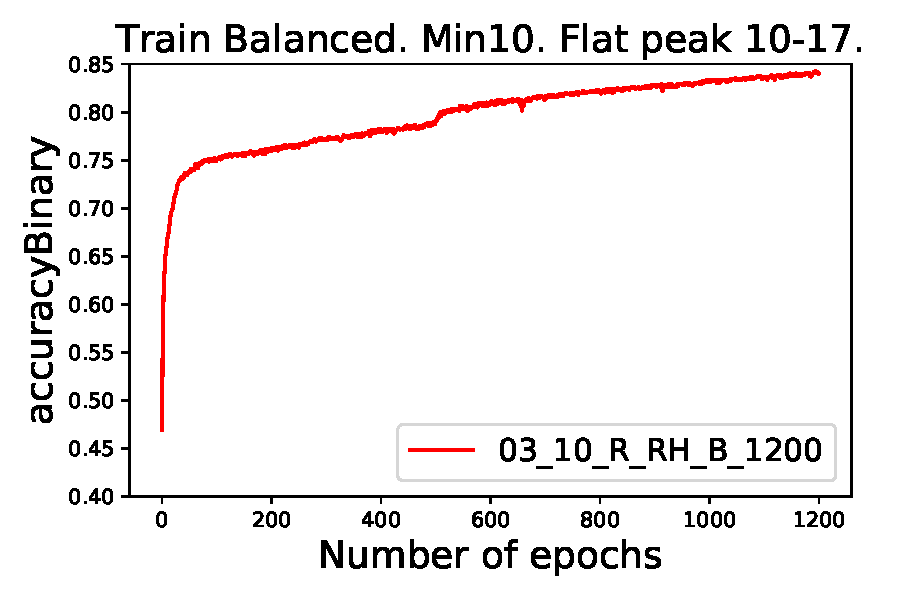
\includegraphics[width=0.45\textwidth]{plots/plot_01_1_overlay_graph_accuracyBinary_Train.pdf}
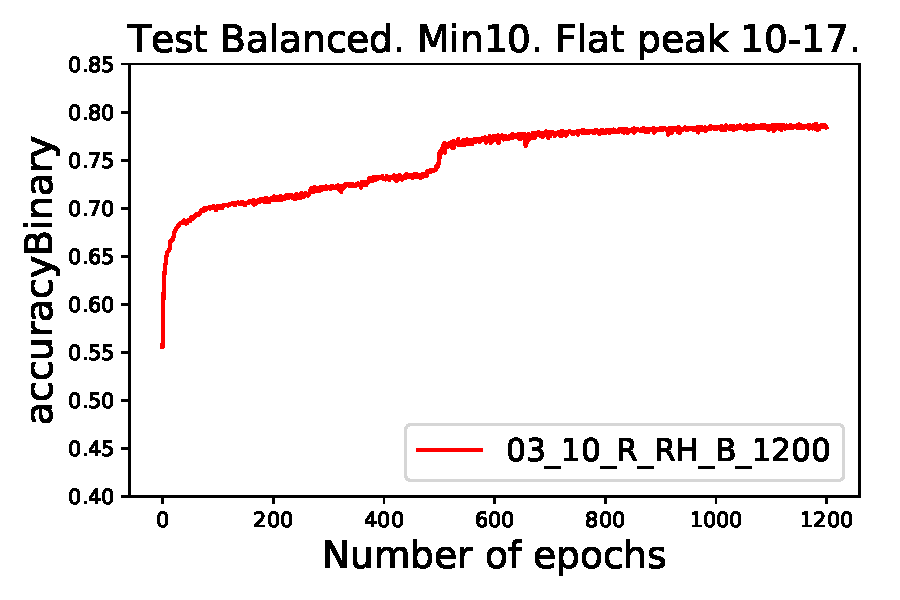
\includegraphics[width=0.45\textwidth]{plots/plot_01_1_overlay_graph_accuracyBinary_Test.pdf}\\
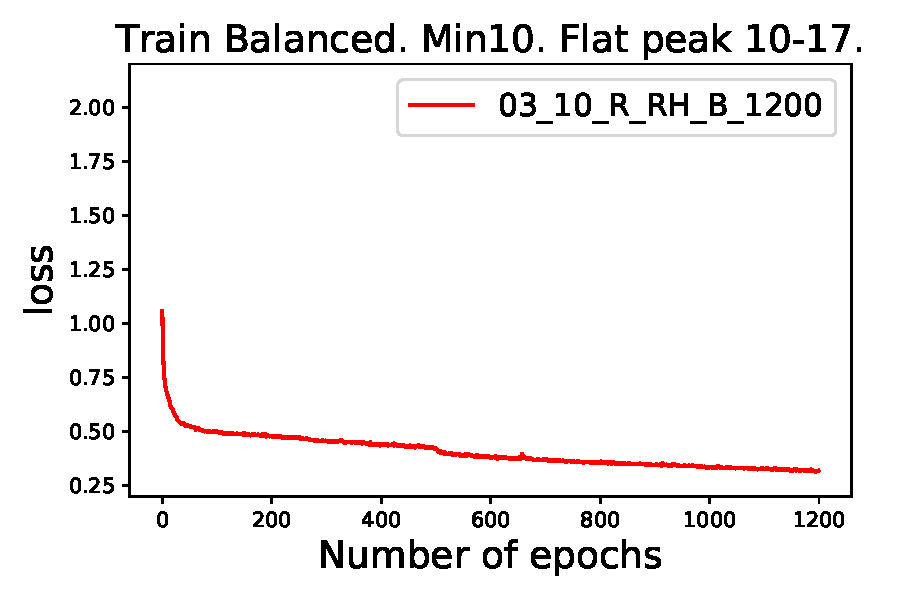
\includegraphics[width=0.45\textwidth]{plots/plot_01_1_overlay_graph_loss_Train.pdf}
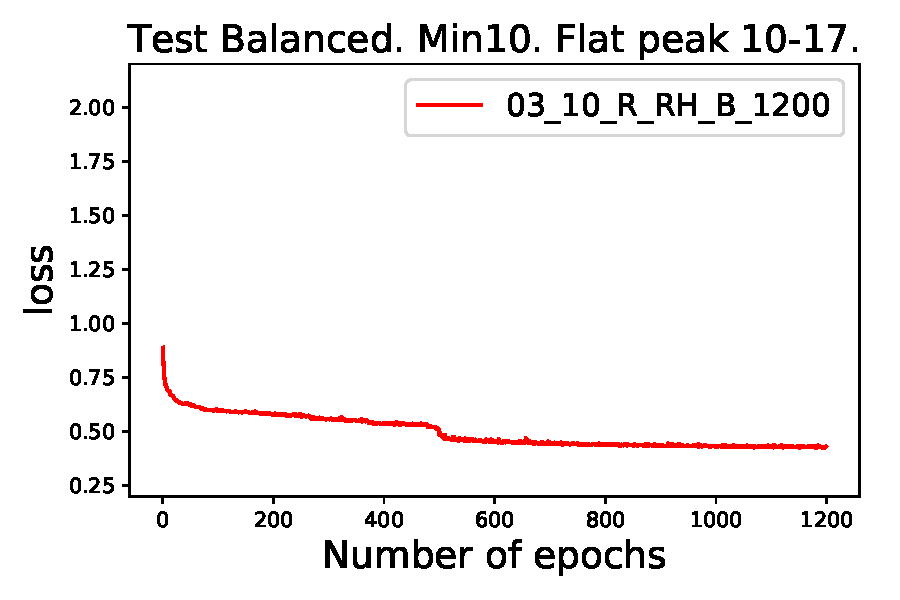
\includegraphics[width=0.45\textwidth]{plots/plot_01_1_overlay_graph_loss_Test.pdf}\\
\caption{Binary accuracy and loss, as resulted directly from training in Keras and Tensorflow. Note that while Train is balanced, Test is also balanced, as it would be too slow to have it unbalanced.}
\label{fig:AccuracyLoss}
\end{figure}

\section{Hit-Level Metrics}
\label{sec:HitLevelMetrics}

In this section the metrics at the hit-level are studied. A bucket is made of 20 hits. Figure~\ref{fig:OutputOutputPredicted1D} presents at the top the distribution of the number of positive hits ($\nbPositiveHit$), at the bottom the distribution of the number of hits predicted to be positive, with Train on the left and Test on the right. The distributions are normalised, so their shapes can be compared. The number of events used in Train relative to Test is 7 to 3. Furthermore, the Train dataset is balanced, keeping only a tiny subset of the buckets, while the Test dataset is unbalanced, keeping all of its buckets. In both datasets all values of $\nbPositiveHit < 10$ are set artificially to 0, considering there was no hit belonging to an interesting particle. Furthermore, the Train dataset is balanced, so that buckets with $\nbPositiveHit$ between 10 and 17 are eliminated, so that equal numbers of buckets for each \nbPositiveHit~remain. Since the distribution is falling (as seen in the Test plot), all values take the lower value of the bin 17. Values 18-20 are left unchanged, as they are too small. Values 18-20 are left unchanged, as they are too small.

\ \\Tests were done with values varying from 14 to 20, but 17 had by far the best outcome. Lower than 17 would not have a training distribution flat enough. Higher than 17 would leave very few buckets to train on. 

\ \\At the bottom of Figure~\ref{fig:OutputOutputPredicted1D} there are the equivalent plots after the prediction using our model. The training is quite solid. There is a tall bin at $\nbPositiveHit=0$, followed by virtually empty bins, and the distributions starts to grow at $\nbPositiveHit=10$, just as in the desired output distribution. For the higher bins, the relative shape does not agree fully to the desired output. For Train, instead of being flat, the distribution increases with larger \nbPositiveHit. For Test it decreases as expected, but not nearly as fast. Overall, however, the model behaves quite well, relative to many other hyper-parameter settings tried.


\begin{figure}[t]
\centering
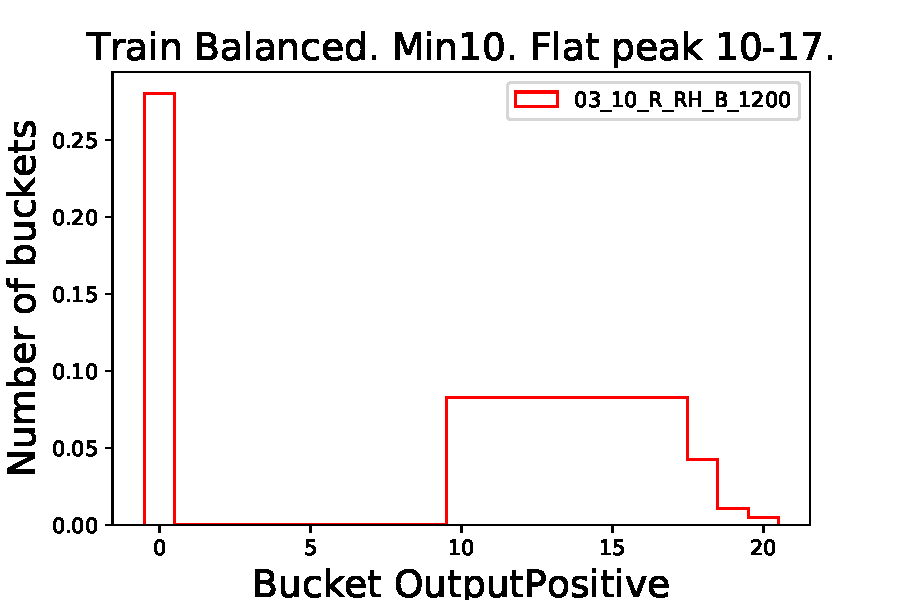
\includegraphics[width=0.45\textwidth]{plots/plot_02_1_overlay_histo_OutputPositive_Train.pdf}
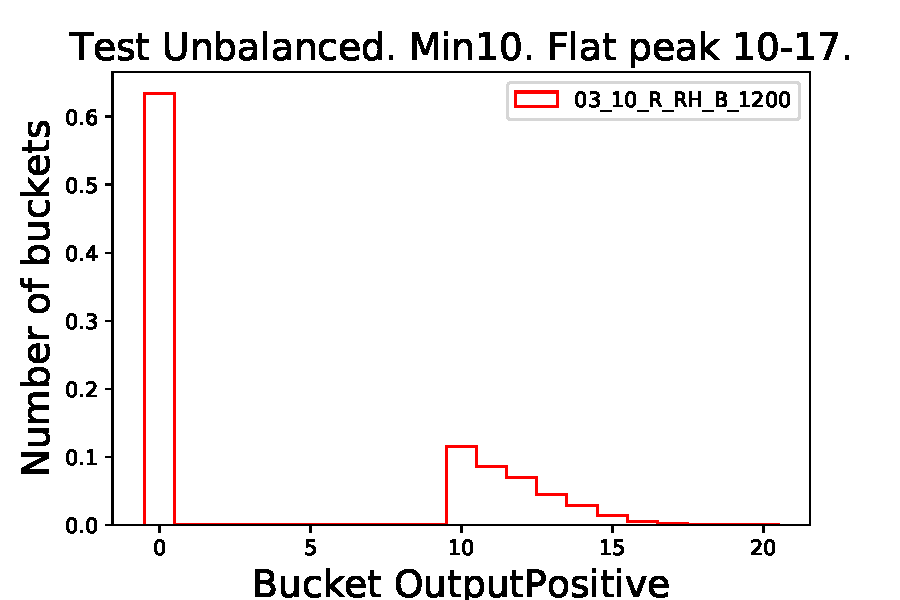
\includegraphics[width=0.45\textwidth]{plots/plot_02_1_overlay_histo_OutputPositive_Test.pdf}\\
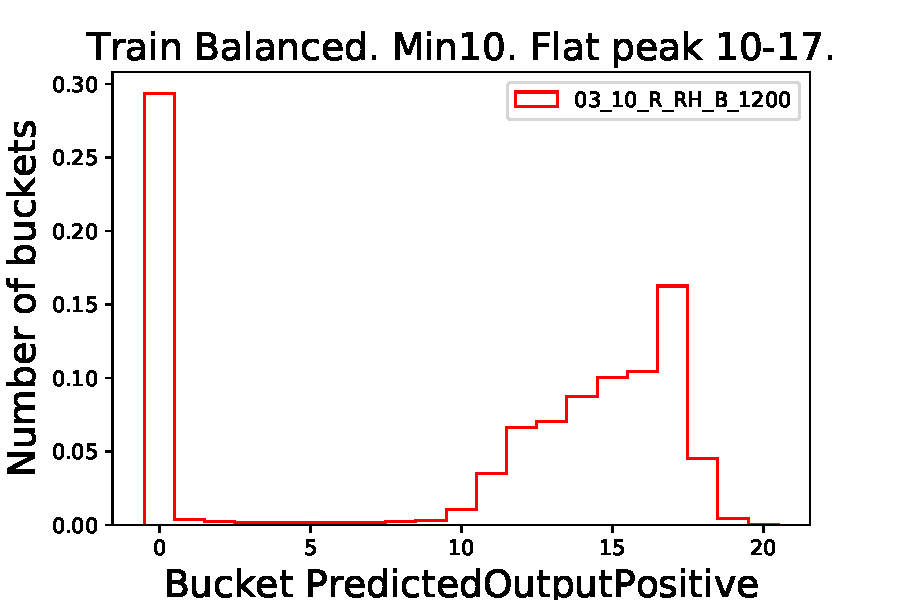
\includegraphics[width=0.45\textwidth]{plots/plot_02_1_overlay_histo_PredictedOutputPositive_Train.pdf}
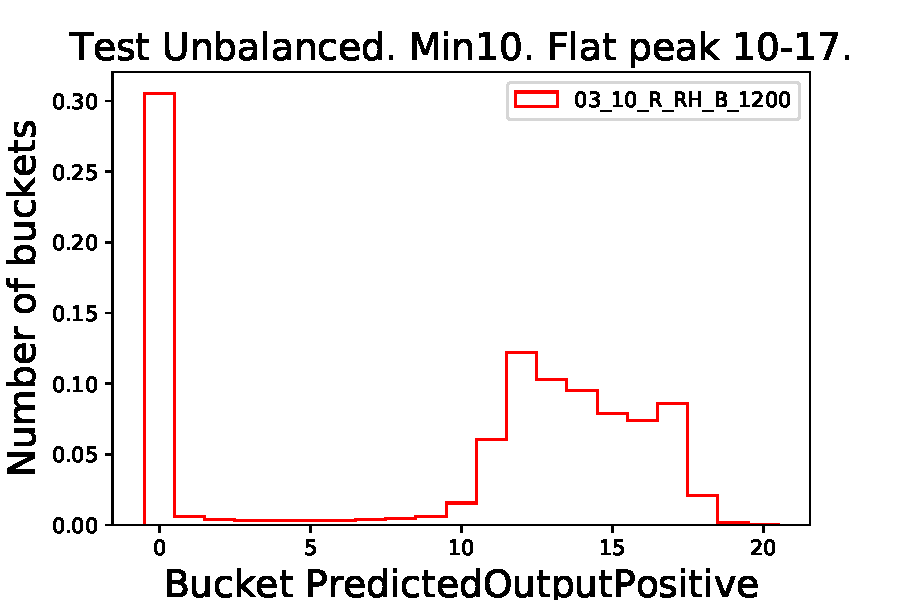
\includegraphics[width=0.45\textwidth]{plots/plot_02_1_overlay_histo_PredictedOutputPositive_Test.pdf}\\
\caption{Output and output predicted 1D. Older ones have a sharp peak, the new ones are more flat.}
\label{fig:OutputOutputPredicted1D}
\end{figure}

\ \\Figure~\ref{fig:OutputOutputPredicted2D} presents the 2D distributions of the output predicted vs output in terms of number of positive hits. The color coding is proportional to the number of entries in the 2D histogram. As expected, there is a peak at (0, 0), meaning events with exactly zero number of positive hits (after the move of all values smaller than 10 to 0), and that are also predicted to have exactly zero. There is nothing between 1 and 9. And for values $\ge 10$, there is a diagonal, as expected for the Train balanced. For the Test unbalanced, it is harder to see. But indeed most entries are in the top left corner of this region, as expected.


\begin{figure}[t]
\centering
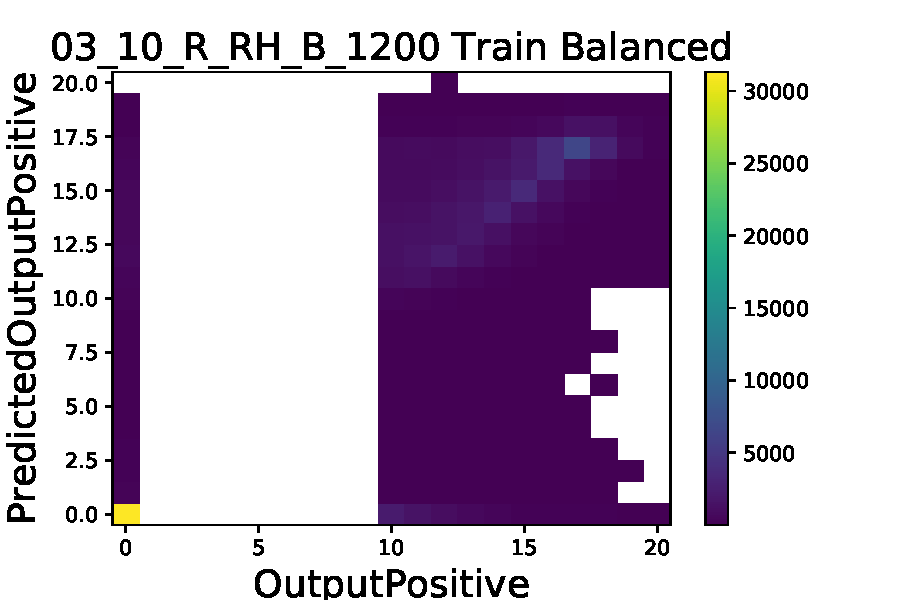
\includegraphics[width=0.45\textwidth]{plots/plot_04_1_overlay_histo2D_OutputPositive_PredictedOutputPositive_03_10_R_RH_B_1200_Train.pdf}
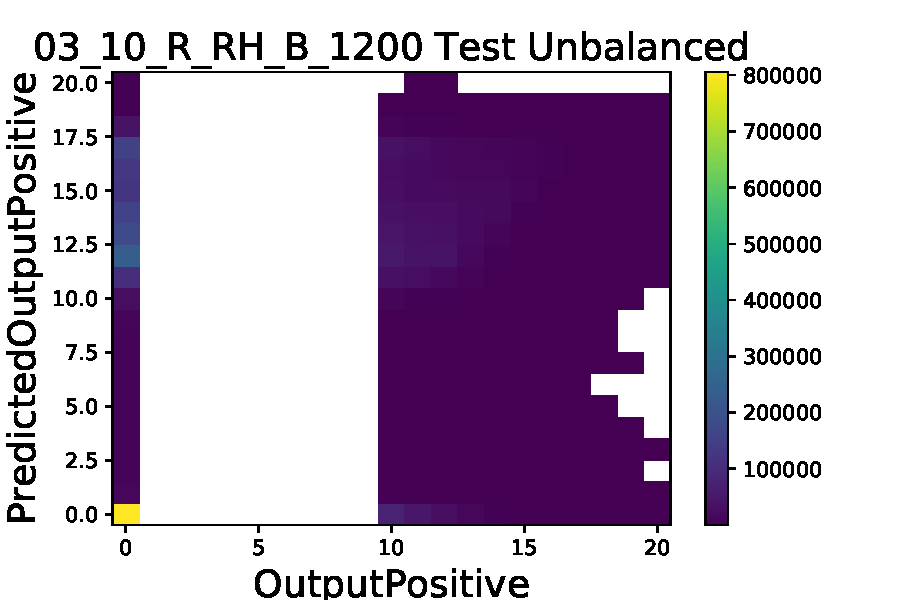
\includegraphics[width=0.45\textwidth]{plots/plot_04_1_overlay_histo2D_OutputPositive_PredictedOutputPositive_03_10_R_RH_B_1200_Test.pdf}\\
\caption{Output and output predicted 2D. In Train balanced, a diagonal is seen. In Test unbalanced it's harder to see.}
\label{fig:OutputOutputPredicted2D}
\end{figure}

\ \\From these plots it can be concluded that in the balanced dataset (Train and Test) a diagonal can be nicely seen. In the Test unbalanced it is harder to see, but still values look relatively flat in 1D. 

\ \\Figure~\ref{fig:FiguresOfMerit1} presents figures of merit at hit level for each \volumeID~in the detector. By looping over all buckets and all hits, both the true and predicted output labels for each hit are known. It results if the hit is TP (True Positive), FP (False Positive), FN (False Negative), or TN (True Negative). The number of hits in these four categories in each \volumeID~is counted. From these for each \volumeID~there are estimated the figures of merit of accuracy, precision, recall, predicted output negative and true negative rate. They all need to be as high as possible, ideally 1. As it is impossible for one model to satisfy all criteria, as known from the bias-variance trade-off, a model with overall good performance across all categories is chosen.

\begin{figure}[t]
\centering
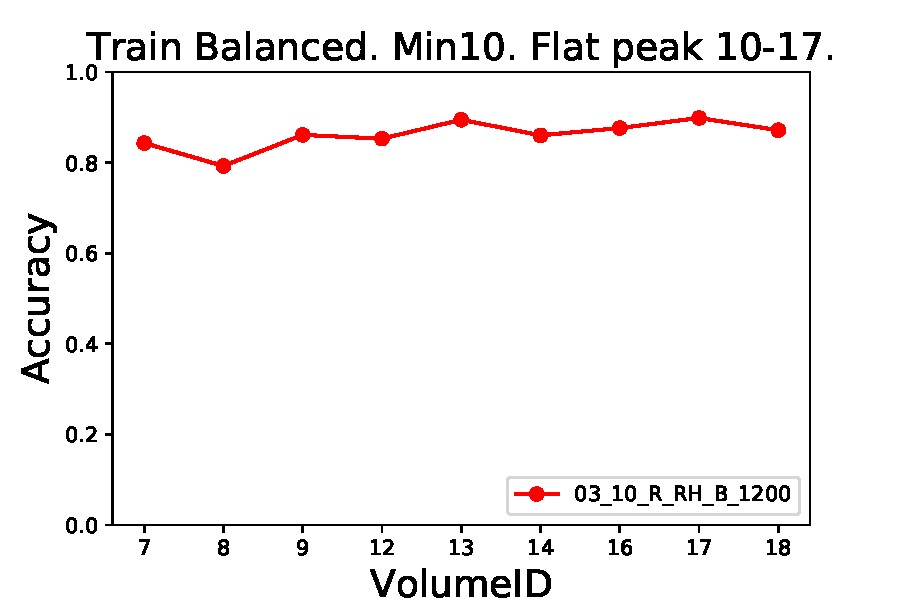
\includegraphics[width=0.45\textwidth]{plots/plot_03_1_overlay_graph_Accuracy_VolumeID_Train.pdf}
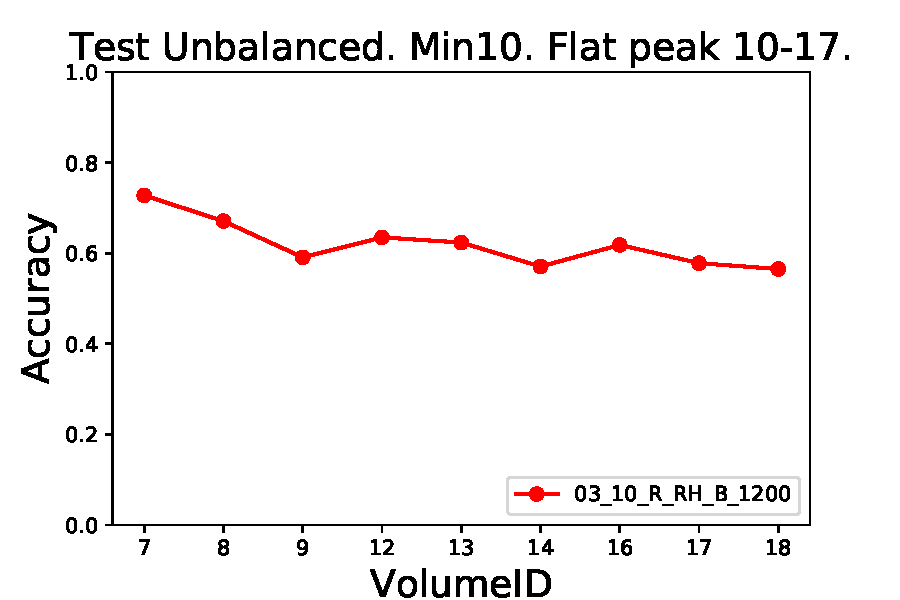
\includegraphics[width=0.45\textwidth]{plots/plot_03_1_overlay_graph_Accuracy_VolumeID_Test.pdf}\\
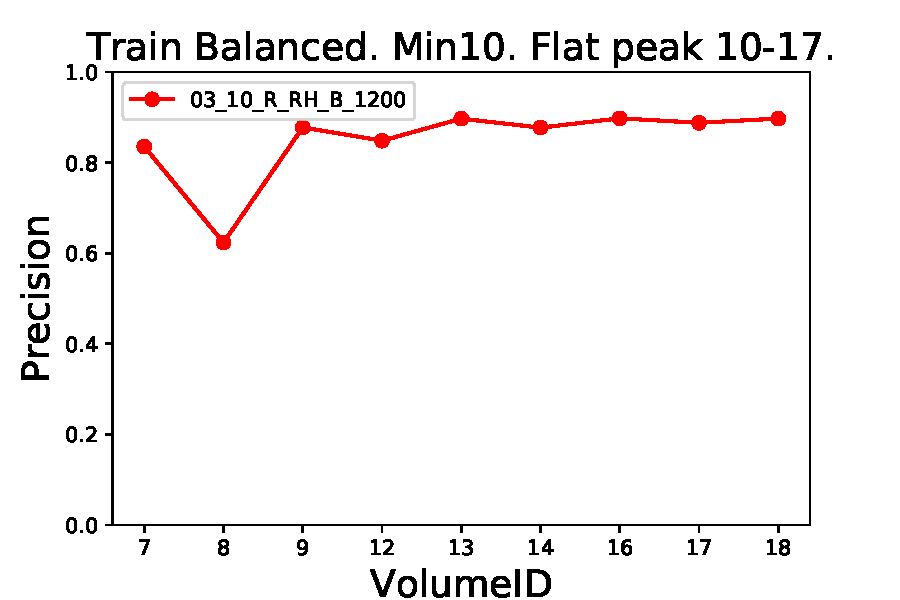
\includegraphics[width=0.45\textwidth]{plots/plot_03_1_overlay_graph_Precision_VolumeID_Train.pdf}
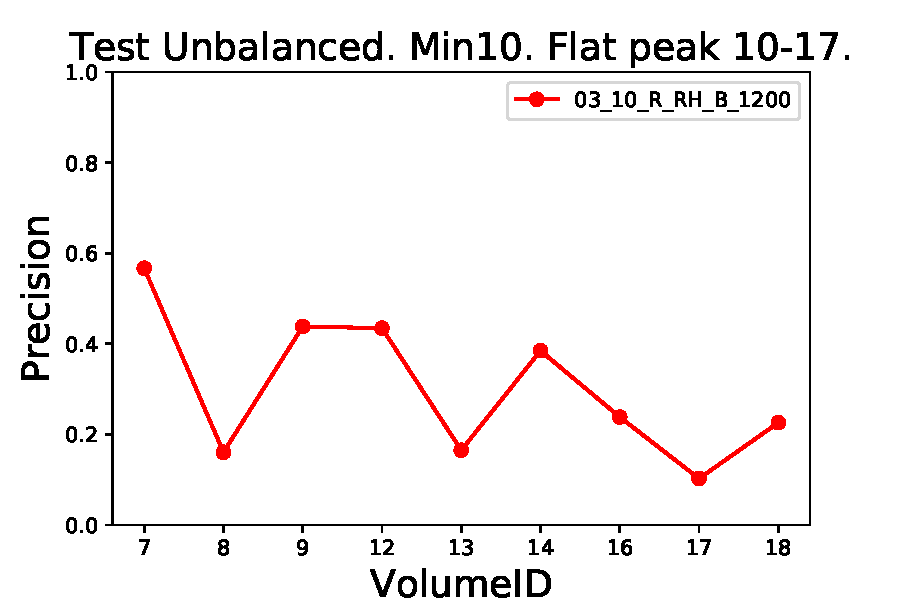
\includegraphics[width=0.45\textwidth]{plots/plot_03_1_overlay_graph_Precision_VolumeID_Test.pdf}\\
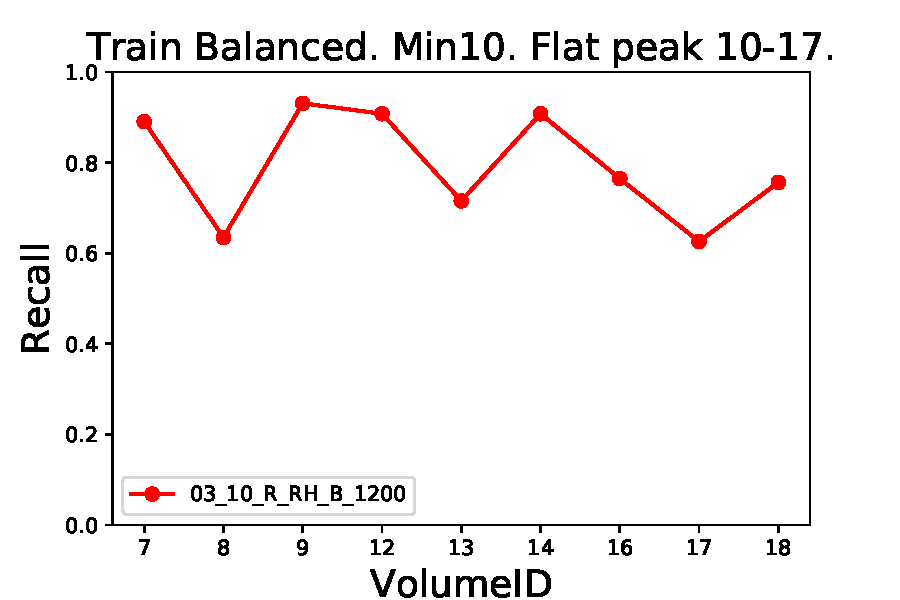
\includegraphics[width=0.45\textwidth]{plots/plot_03_1_overlay_graph_Recall_VolumeID_Train.pdf}
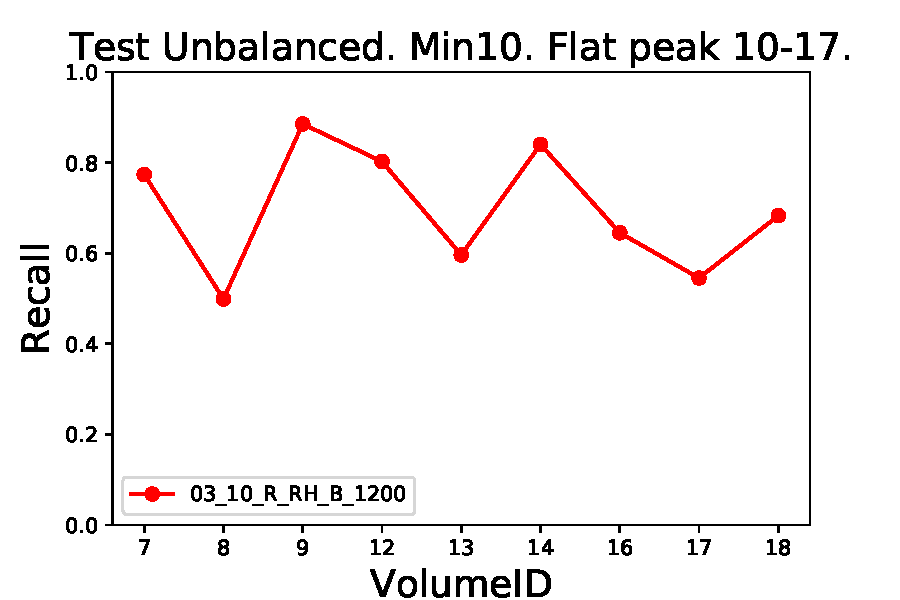
\includegraphics[width=0.45\textwidth]{plots/plot_03_1_overlay_graph_Recall_VolumeID_Test.pdf}\\
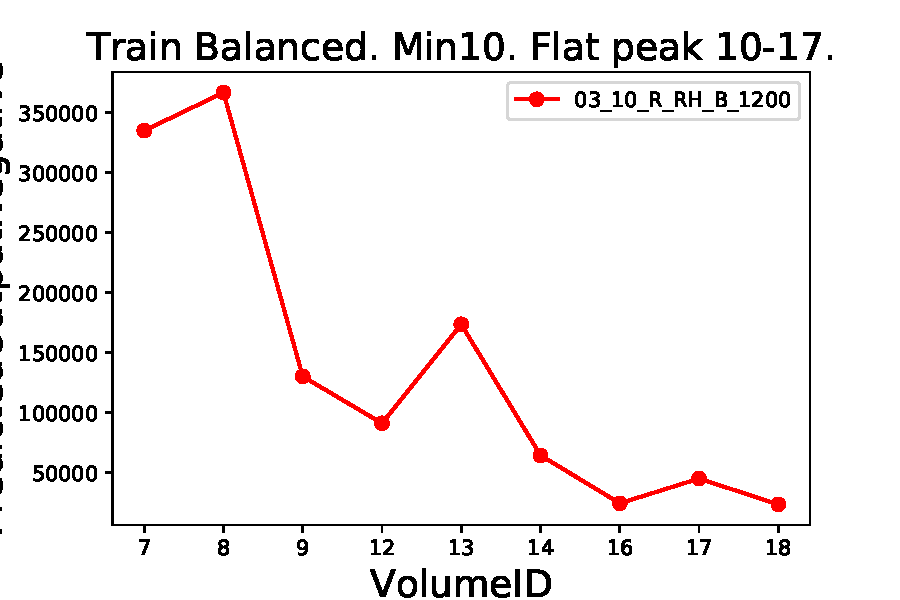
\includegraphics[width=0.45\textwidth]{plots/plot_03_1_overlay_graph_PredictedOutputNegative_VolumeID_Train.pdf}
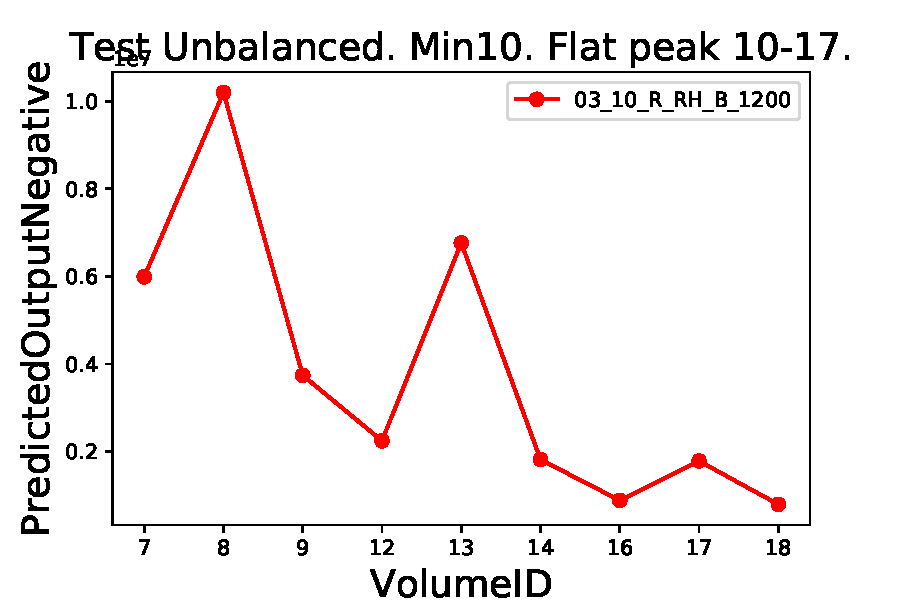
\includegraphics[width=0.45\textwidth]{plots/plot_03_1_overlay_graph_PredictedOutputNegative_VolumeID_Test.pdf}\\
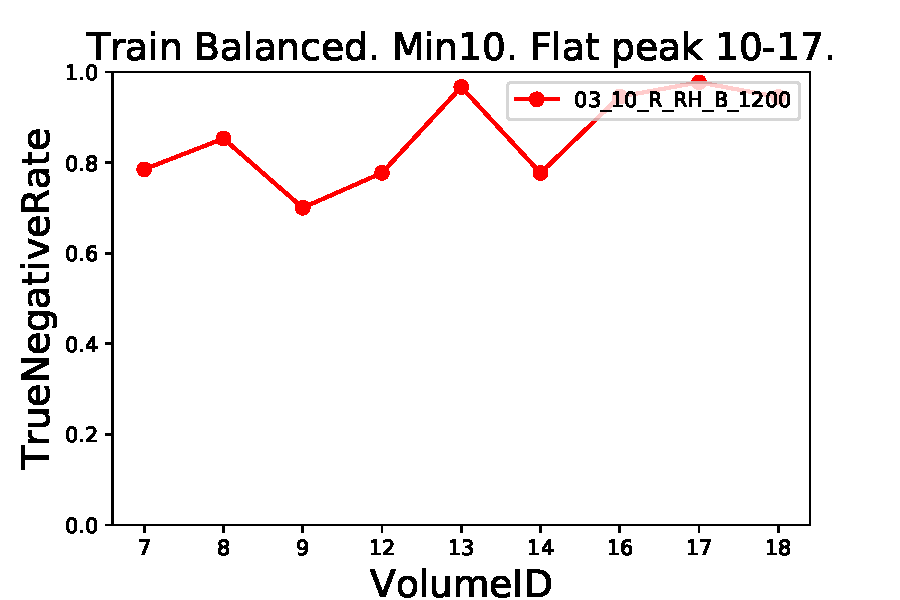
\includegraphics[width=0.45\textwidth]{plots/plot_03_1_overlay_graph_TrueNegativeRate_VolumeID_Train.pdf}
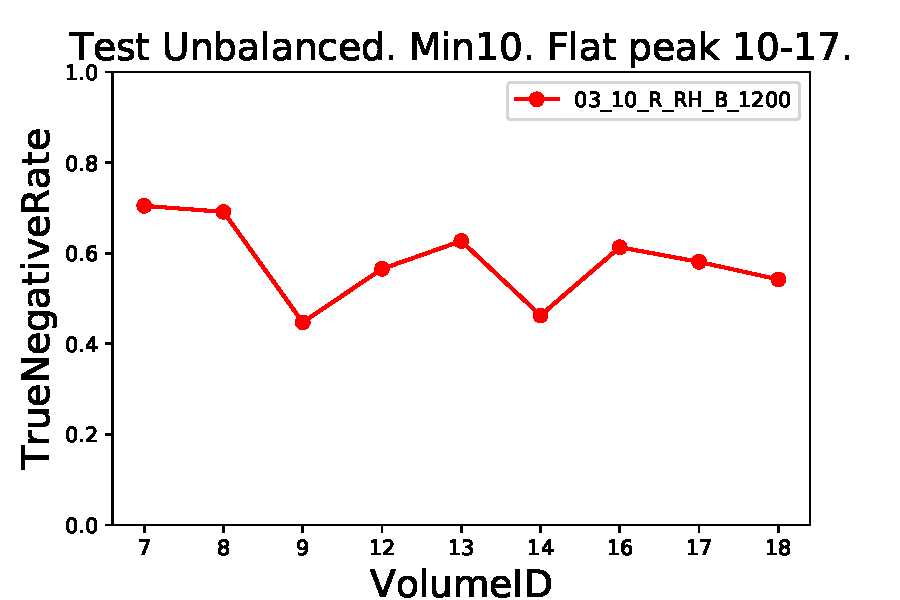
\includegraphics[width=0.45\textwidth]{plots/plot_03_1_overlay_graph_TrueNegativeRate_VolumeID_Test.pdf}\\
\caption{Accuracy, precision, recall, predicted output negative, true negative rate. Train (left) and Test (right). }
\label{fig:FiguresOfMerit1}
\end{figure}


\section{Particle-Level Metrics}
\label{sec:ParticleLevelMetrics}

Two numpy arrays of dimension two are used: the true output and the output predicted by the model. Each row represents a bucket. There are 20 columns, representing the 20 hits. A for loop over buckets is made. For each bucket a loop over hits is made. Each hit has a value of -1 or +1 for the output and for the predicted output. For the current bucket, the number of hits that are positive (\nbPositiveHit) is counted. A count is also made for those that are both positive and in addition predicted to also be positive (\nbTruePositiveHit). A bucket with $\nbPositiveHit \ge10$ is considered to contain a truth particle. If in addition the bucket has also $\nbTruePositiveHit /\nbPositiveHit > 80\%$, it is considered to also have reconstructed correctly that particle. A count is made of the buckets that have a truth particle, and then those that both have a truth particle and have reconstructed it. The efficiency to reconstruct a particle ($\eff = \nbParticleReco / \nbParticleTruth$) is 84.2\% for Train and 71.3\% for Test. Detailed results are summarized in Table~\ref{tab:ParticleReconstructionEfficiency}.

\begin{table}[h!]
\centering
  \resizebox{\textwidth}{!}{
    \begin{tabular}{|l|l|l|l|l|} % <-- Alignments: 1st column left, 2nd middle and 3rd right, with vertical lines in between
      \hline
      Sample & \eff & \nbBucket & \nbParticleTruth & \nbParticleReco \\
      \hline
      Train Balanced & 84.2\% & 130k &  94k & 79k \\
      Test Balanced & 74.9\%  & 62k & 45k & 34k \\
      Test Unbalanced & 71.3\% & 3219k & 1178k & 840k \\
      \hline
    \end{tabular}
  }
\caption {Particle reconstruction efficiency results.}
\label{tab:ParticleReconstructionEfficiency}
\end{table}
